\documentclass[11pt]{article}

\def\chapitre{13}
\def\pagetitle{Suites réelles : la pratique.}

\input{/home/theo/MP2I/setup.tex}

\begin{document}

\input{/home/theo/MP2I/title.tex}

\renewcommand*{\0}{\mathbbm{0}}

\thispagestyle{fancy}

\setcounter{section}{-1}

Ce chapitre sera complété par le cours \bf{Suites réelles : la théorie}, dans lequel sera donnée une définition rigoureuse de la notion de suite convergente, ainsi que des preuves pour les théorèmes énoncés ici. On souhaite d'abord se focaliser sur les méthodes et les exemples, et notamment sur les deux outils fondamentaux que sont le théorème d'éncadrement, et le théorème des gendarmes.

\section{Qu'est-ce qu'une suite ?}

\begin{defi}{}{}
    On appelle \bf{suite réelle} une application de $\N$ dans $\R$. Ainsi, $\R^\N$ est l'ensemble des suites réelles.
\end{defi}

Une suite numérique est donc une suite de nombres. On s'intéressera un jour à des suites de matrices, des suites de fonctions...

\begin{nota}{}{}
    Soit une suite $u:\N\to\R$. Pour tout $n\in\N$, le nombre $u(n)$ est noté $u_n$ et appelé \bf{terme général} de la suite, ou terme de rang $n$. La suite $u$ est notée $(u_n)_{n\geq0}$ ou $(u_n)_{n\in\N}$ ou $(u_n)$.
\end{nota}

\section{Calculs de limites.}

\subsection{Limites usuelles.}

\begin{prop}{Limite d'une puissance de $n$.}{}
    Soit $\a\in\R$. La suite $(n^\a)_{n\in\N^*}$ a une limite, qui vaut
    \begin{equation*}
        \lim_{n\to+\infty} n^\a = \begin{cases}
            +\infty &\nt{si } \a>0\\
            1 &\nt{si } \a=0\\
            0 &\nt{si } \a<0
        \end{cases}
    \end{equation*}
\end{prop}

\begin{prop}{Limite d'une suite géométrique.}{}
    Soit $q\in\R$. On a
    \begin{equation*}
        \lim_{n\to+\infty} q^n = \begin{cases}
            +\infty &\nt{si } q>1\\
            1 &\nt{si } q=1\\
            0 &\nt{si } q\in]-1,1[\\
            \nt{n'existe pas} &\nt{si } q\leq-1
        \end{cases}
    \end{equation*}
\end{prop}

\begin{prop}{Croissances comparées.}{}
    Soit $\a\in\R_+^*, p>1$ et $q\in]-1,1[$. On a les limites suivantes:
    \begin{equation*}
        \lim_{n\to+\infty}\frac{n^\a}{p^n}=0, \quad\et\quad \lim_{n\to+\infty}n^\a q^n = 0.
    \end{equation*}
    \emph{Une suite géométrique l'emporte toujours sur une puissance de $n$}.
\end{prop}

\subsection{Opérations algébriques et limits.}

\quad Pour énoncer les proposition suivantes, on se donne $(u_n)$ et $(v_n)$ deux suites réelles admettant une limite, finie ou infinie, aisni que deux réels $l$ et $l'$. Les tableaux donnent les limites de suites construites par opérations sur $(u_n)$ et $(v_n)$. La mention F.I. (<< forme indéterminée >>) signale que l'on ne peut rien dire en général.

\begin{prop}{Limite d'une somme.}{}
    Si $(u_n)$ et $(v_n)$ sont deux suites convergentes, alors $(u_n+v_n)$ l'est aussi et la limite de la somme est la somme des limites.
    \begin{eqnarray*}
        \begin{array}{|c|c|c|c|c|}
            \hline
            \lim u_n & l & +\infty & -\infty & +\infty\\
            \hline
            \lim v_n & l' & l'\ou+\infty & l'\ou-\infty & -\infty\\
            \hline
            \lim(u_n+v_n) & l+l' & +\infty & -\infty & \text{F.I.}\\
            \hline
        \end{array}
    \end{eqnarray*}
\end{prop}

\begin{prop}{Limite d'un produit.}{}
    \begin{eqnarray*}
        \begin{array}{|c|c|c|c|c|c|c|c|}
            \hline
            \lim u_n & l & +\infty & + \infty & +\infty & -\infty & -\infty & -\infty\\
            \hline
            \lim v_n & l' & l'>0\ou+\infty&l'<0\ou-\infty&0&l'>0\ou+\infty&l'<0\ou-\infty&0\\
            \hline
            \lim(u_nv_n) & ll' & +\infty & -\infty & \text{F.I.} & -\infty & +\infty & \nt{F.I}.\\
            \hline
        \end{array}
    \end{eqnarray*}
\end{prop}

\begin{prop}{Limite et inverse.}{}
    Dans tous les cas ci-dessus, la suite $(u_n)$ ne s'annule pas à partir d'un certain rang.
    \begin{eqnarray*}
        \begin{array}{|c|c|c|c|c|c|}
            \hline
            \lim u_n & l\in\R^* & 0_+ & 0_- & +\infty & -\infty\\
            \hline
            \lim\frac{1}{u_n} & \frac{1}{l} & +\infty & -\infty & 0_+ & 0_-\\
            \hline
        \end{array}
    \end{eqnarray*}
\end{prop}

\begin{prop}{Limite d'un quotient.}{}
    Dans tous les cas ci-dessus, la suite $(v_n)$ ne s'annule pas à partir d'un certain rang.
    \begin{eqnarray*}
        \begin{array}{|c|c|c|c|c|c|c|c|c|c|}
            \hline
            \lim u_n & l & l & l & l & 0 & +\infty & +\infty & \pm \infty\\
            \hline
            \lim v_n & l'\in\R^* & \pm \infty & 0_+ & 0_- & 0 & l>0 \ou 0_+ & l < 0 \ou 0_- & \pm \infty\\
            \hline
            \lim\frac{u_n}{v_n} & \frac{l}{l'} & 0 & +\infty & -\infty & \text{F.I.} & +\infty & -\infty & \nt{F.I}.\\
            \hline
        \end{array}
    \end{eqnarray*}
\end{prop}

\section{Existence d'une limite : deux outils fondamentaux.}

Dans cette partie, on énonce et on illustre les deux outils principaux qui pourront être mobilisés dans la pratique pour prouver qu'une suite converge : le théorème d'encadrement et le théorème de la limite monotone. Ces résultats reposent sur des inégalités : toutes les suites ici seront \bf{réelles}.

\subsection{L'encadrement.}

\begin{thm}{d'encadrement, ou des gendarmes.}{}
    Soient trois suites réelles $(g_n)$, $(u_n)$ $(d_n)$ telles que $\forall n \in \N \quad g_n \leq u_n \leq d_n$.\\
    Si de surcroît, $(g_n)$ et $(d_n)$ convergent vers la même limite $l\in \R$, alors
    \begin{equation*}
        (u_n) \nt{ est convergente \quad et \quad} \lim u_n = l.
    \end{equation*}
\end{thm}

\begin{ex}{utiliser le théorème d'encadrement.}{}
    Montrer que la suite $(u_n)$ de terme général $\displaystyle\frac{\lf \sqrt{n} - 1 \rf}{\lf \sqrt{n} + 1 \rf}$ converge et préciser sa limite.
    \tcblower
    Pour $n\in\N^*$, $\sqrt{n}-2\leq\lf \sqrt{n} - 1 \rf \leq \sqrt{n}-1$ et $\sqrt{n}\leq \lf \sqrt{n} + 1 \rf \leq \sqrt{n} + 1$. Ainsi :
    \begin{equation*}
        \frac{\sqrt{n}-2}{\sqrt{n}+1} \leq u_n \leq \frac{\sqrt{n}-1}{\sqrt{n}} \quad\nt{alors}\quad \frac{1-\frac{2}{\sqrt{n}}}{1+\frac{1}{\sqrt{n}}}\leq u_n \leq 1-\frac{1}{\sqrt{n}}
    \end{equation*}
    On a $(u_n)$ encadrée par deux suites convergentes vers $1$, donc $u_n\to1$ par théorème des gendarmes.
\end{ex}

\begin{meth}{Majorer la distance par une suite qui tend vers 0.}{}
    Pour montrer qu'une suite $(u_n)$ tend vers un réel $l$, il suffit d'obtenir une majoration du type
    \begin{equation*}
        |u_n-l|\leq v_n
    \end{equation*}
    où $(v_n)$ est une suite qui tend vers 0.\n
    En particulier, pour montrer qu'une suite tend vers 0, il suffit de majorer sa valeur absolue par une suite qui tend vers 0.
\end{meth}

\begin{meth}{Encadrer une somme, une intégrale.}{}
    Pour encadrer une somme,\\
    \quad on propose un encadrement pour chaque terme,\\
    \quad puis on somme les inégalités.\\
    \emph{Parfois intéressant : majorer/minorer chaque terme par le plus grand/petit d'entre eux.}\n
    Pour encadrer une intégrale,\\
    \quad on propose un encadrement pour la fonction intégrée,\\
    \quad puis intègre l'inégalité (croissance de l'intégrale : bornes bien rangées parmi les hypothèses).\n
    L'inégalité triangulaire est un outil pour majorer la valeur absolue d'une somme ou d'une intégrale.
\end{meth}

\begin{ex}{Montrer qu'une suite tend vers 0 en écrasant la valeur absolue.}{}
    Démontrer que les suites de terme général 0 ci-dessous tendent vers 0 :
    \begin{equation*}
        u_n=\frac{n\sin(n)}{n+2^n}; \qquad v_n = \sum_{k=n+1}^{2n}\frac{(-1)^k}{k^2}; \qquad w_n=\int_0^1x^n\sin(nx)\arctan(n^x)\dx
    \end{equation*}
    \tcblower
    Soit $n\in\N$.\\
    --- On a $\displaystyle|u_n|=\left|\frac{n\sin(n)}{n+2^n}\right|=\frac{n|\sin(n)|}{n+2^n}\leq\frac{n}{n+2^n}$ car $|\sin(n)|\leq1$. Or $\displaystyle\frac{n}{2^n}\to0$ par croissances comparées.\\
    Donc $\displaystyle\frac{n}{n+2^n}\to0$ donc $|u_n|\to0$ donc $u_n\to0$.\n
    --- On a $\displaystyle|v_n|=\left|\sum_{k=n+1}^{2n}\frac{(-1)^k}{k^2}\right|\leq\sum_{k=n+1}^{2n}\frac{1}{k^2}\leq\sum_{k=n+1}^{2n}\frac{1}{(n+1)^2}\leq\frac{n}{(n+1)^2}\leq\frac{1}{n(1+\frac{1}{n})^2}\to0$\n
    --- On a $\displaystyle|w_n|=\left|\int_0^1x^n\sin(nx)\arctan(n^x)\dx\right|\leq\frac{\pi}{2}\int_0^1x^n\dx=\frac{\pi}{2}\cdot\frac{1}{n+1}\to0$.
\end{ex}

\begin{ex}{utiliser le théorème d'encadrement avec des sommes.}{}
    Convergence et limite des suites $u$ et $v$ de terme général
    \begin{equation*}
        u_n = n\sum_{k=n+1}^{2n}\frac{1}{n^2+k} \quad\et\quad v_n=\frac{1}{n^2}\sum_{k=1}^n\lf k\pi \rf.
    \end{equation*}
    \tcblower
    Soit $n\in\N$. Soit $k\in \lb n+1,2n\rb$.\\
    $\bullet$ On a $\displaystyle\frac{1}{n^2+2n}\leq\frac{1}{n^2+k}\leq\frac{1}{n^2+n+1}$ donc $\displaystyle\frac{n^2}{n^2+2n}\leq n\sum_{k=n+1}^{2n}\frac{1}{n^2+k}\leq\frac{n^2}{n^2+n+1}$.\\
    Par encadrement, $u_n\to1$.\\
    $\bullet$ Soit $k\in \lb1,n\rb$. On a $k\pi-1\leq\lf k\pi \leq k\pi$ donc $\displaystyle\sum_{k=1}^nk\pi-n\leq\sum_{k=1}^n\lf k\pi \rf \leq \sum_{k=1}^nk\pi$. On multiplie par $\frac{1}{n^2}$:
    \begin{equation*}
        \frac{n(n+1)}{2}\cdot\frac{\pi}{n^2}-\frac{1}{n} \leq v_n \leq \frac{\pi}{n^2}\cdot\frac{n(n+1)}{2}.
    \end{equation*}
    Par encadrement, $v_n\to \frac{\pi}{2}$.
\end{ex}

\begin{prop}{de minoration, de majoration.}{}
    Soient $(u_n)$ et $(v_n)$ deux suites réelles.
    \begin{itemize}
        \item Si $\forall n\in \N, ~ u_n \leq v_n$ et $u_n\to+\infty$, alors $v_n\to+\infty$.
        \item Si $\forall n\in \N, ~ u_n \leq v_n$ et $v_n\to-\infty$, alors $u_n\to-\infty$.
    \end{itemize}
\end{prop}

\begin{ex}{}{}
    Soit $n\in\N^*$. On pose $\displaystyle u_n=\sum_{k=n+1}^{2n}\frac{1}{\sqrt{k}}$. Démontrer que $u_n\to+\infty$.
    \tcblower
    Soit $k\in\lb n+1, 2n \rb$. On a $\ds\frac{1}{\sqrt{k}}\geq\frac{1}{\sqrt{2n}}$ donc $\ds\sum_{k=n+1}^{2n}\frac{1}{\sqrt{k}}\geq\sum_{k=n+1}^{2n}\frac{1}{\sqrt{2n}}$ donc $\ds u_n\geq\sqrt{\frac{n}{2}}\to+\infty$.
\end{ex}

\pagebreak

\begin{ex}{La série harmonique.}{}
    Pour $n\in\N^*$, on note $\ds H_n=\sum_{k=1}^n\frac{1}{k}$.
    \begin{enumerate}
        \item Pour $k\in\N^*$, justifier que $\ln(1+\frac{1}{k})\leq\frac{1}{k}$.
        \item Démontrer que $H_n\to+\infty$.
    \end{enumerate}
    \tcblower
    \boxed{1.} $\ln$ est concave donc en dessous de sa tangente en 1. Alors $\forall x \in \R^*, ~ \ln(x)\leq x-1$.\\
    En particulier, pour $k\in\N^*$, $\ln(1+\frac{1}{k})\leq\frac{1}{k}$.\\
    \boxed{2.} Soit $n\in\N^*$.
    \begin{align*}
        \sum_{k=1}^n\ln\left(1+\frac{1}{k}\right)\leq\sum_{k+1}^n\frac{1}{k} \quad&\nt{donc}\quad\sum_{k=1}^n\ln\left( \frac{k+1}{k} \right) \leq H_n\\
        &\nt{donc}\quad\sum_{k=1}^n\left( \ln(k+1) - \ln(k) \right) \leq H_n\\
        &\nt{donc}\quad\ln(n+1)\cancel{-\ln(1)}\leq H_n
    \end{align*}
    Or $\ln(n+1)\to+\infty$ donc $H_n$ aussi par minoration.
\end{ex}

\subsection{La monotonie.}

\begin{defi}{}{}
    Une suite réelle $(u_n)_{n\geq0}$ est dite
    \begin{center}
        \bf{croissante} si $\forall n\in\N, ~ u_{n+1}\geq u_n$, \qquad \bf{décroissante} si $\forall n \in \N, ~ u_{n+1}\leq u_n$,\\
        \bf{monotone} si elle est croissante ou décroissante.
    \end{center}
\end{defi}

\begin{meth}{}{}
    Soit un entier $n$. Pour comparer deux termes consécutifs $u_n$ et $u_{n+1}$ d'une suite $u$, on pourra
    \begin{itemize}
        \item Examiner le signe de $u_{n+1}-u_n$. C'est bête à dire mais
        \begin{equation*}
            u_{n+1} \geq u_n \iff u_{n+1} - u_n \geq 0.
        \end{equation*}
        \item Dans le cas où la suite est strictement positive, comparer le quotient $\ds\frac{u_{n+1}}{u_n}$ à 1, puisqu'alors
        \begin{equation*}
            u_{n+1} \geq u_n \iff \frac{u_{n+1}}{u_n} \geq 1.
        \end{equation*}
    \end{itemize}
\end{meth}

\begin{defi}{}{}
    Une suite réelle $(u_n)_{n\geq0}$ est
    \begin{center}
        \bf{majorée} si $\exists M\in\R, ~ \forall n \in \N, ~ u_n \leq M$, \qquad \bf{minorée} si $\exists m \in \R, ~ \forall n\in\N, ~ u_n\geq m$,\\
        \bf{bornée} si elle est majorée et minorée.
    \end{center}
\end{defi}

\begin{prop}{Caractérisation des suites bornées.}{}
    Une suite réelle $(u_n)$ est bornée si et seulement si la suite $(|u_n|)$ est majorée.
\end{prop}

\begin{thm}{de la limite monotone}{}
    Toute suite croissante et majorée converge vers une limite finie.\\
    Toute suite croissante et non majorée diverge vers $+\infty$.
\end{thm}

\begin{corr}{}{}
    Toute suite décroissante et minorée converge vers une limite finie.\\
    Toute suite décroissante et non minorée diverge vers $-\infty$.
\end{corr}

\begin{ex}{}{}
    Établir la convergence des suites $u$ et $v$ définies pour tout $n$ par $\ds u_n=\sum_{k=0}^n\frac{1}{k!}\et v_n=2^{-2n}\binom{2n}{n}$.
    \tcblower
    Soit $n\geq3$.\\
    $\bullet$ $u_{n+1}-u_n=\frac{1}{(n+1)!}\geq0$ donc croissante.\\
    Pour $\ds k\geq3,~\frac{1}{k!}\leq\frac{1}{k^2}\leq\frac{1}{k(k-1)}=\frac{1}{k-1}-\frac{1}{k}$ donc $\ds\sum_{k=3}^n\frac{1}{k!}\leq\sum_{k=3}^n\left( \frac{1}{k-1} - \frac{1}{k} \right)=\frac{1}{2}-\frac{1}{n}$.\\
    Ainsi, $\ds\sum_{k=0}^n\frac{1}{k!}\leq 3 - \frac{1}{n} \leq 3$. On a $u$ croissante et majorée, elle converge d'après le TLM.
\end{ex}

\begin{defi}{}{}
    On dit que deux suites $(u_n)$ et $(v_n)$ sont \bf{adjacentes} lorsque
    \begin{itemize}
        \item $(u_n)$ et $(v_n)$ sont monotones de monotonie opposées,
        \item $v_n - u_n \to 0$.
    \end{itemize}
\end{defi}

\begin{thm}{Convergence des suites adjacentes.}{}
    Deux suites adjacentes convergent vers une même limite finie.\\
    Plus précisément, si $(u_n)$ et $(v_n)$ sont deux suites adjacentes, ($u$ croissante et $v$ décroissante) alors elles convergent vers une même limite finie $l\in\R$. De plus,
    \begin{equation*}
        \forall n \in \N, ~ u_n \leq l \leq v_n.
    \end{equation*}
\end{thm}

\begin{ex}{}{}
    Soient les suites réelles $(u_n)_{n\geq1}$ et $(v_n)_{n\geq1}$ définies par
    \begin{equation*}
        \forall n \geq 1 \quad u_n = \sum_{k=0}^n\frac{1}{k!} \quad\et\quad v_n = \sum_{k=0}^n\frac{1}{k!} + \frac{1}{nn!}
    \end{equation*}
    \begin{enumerate}
        \item Démontrer que $(u_n)$ et $(v_n)$ convergent vers une même limite finie.
        \item On admet que $e=\lim u_n$. Démontrer que $e\notin\Q$.
    \end{enumerate}
    \tcblower
    Soit $n\in\N^*$.\\
    \boxed{1.}\\
    $\bullet$ $\ds u_{n+1} - u_n = \frac{1}{(n+1)!}\geq0$ donc $(u_n)$ est croissante.\\
    $\bullet$ $\ds v_{n+1}-v_n = \frac{1}{(n+1)!} + \frac{1}{(n+1)(n+1)!} - \frac{1}{nn!}=...=-\frac{1}{n!n(n+1)}\leq0$ donc $(v_n)$ est décroissante.\\
    $\bullet$ $v_n - u_n = \frac{1}{nn!}\to0$. Ainsi, les suites $u$ et $v$ sont adjacentes, elles convergent vers une même limite finie.\n
    \boxed{2.} Supposons $e\in\Q$, $\ds \exists p,q\in\N^*\mid e=\frac{p}{q}$. De plus, $u_n < e < v_n$ par monotonies strictes. Ainsi :
    \begin{equation*}
        u_q < e < v_q \quad\nt{donc}\quad \sum_{k=0}^q\frac{1}{k!}<\frac{p}{q}<\sum_{k=0}^q\frac{1}{k!}+\frac{1}{q!q} \quad\nt{donc}\quad \sum_{k=0}^q\frac{q!}{k!}<p(q-1)!<\sum_{k=0}^q\frac{q!}{k!}+\frac{1}{q}
    \end{equation*}
    Notons $\ds N=\sum_{k=0}^q\frac{q!}{k!}\in\N$ car somme d'entiers. Alors $N<p(q-1)!<N+1$.\\
    Or $p(q-1)!\in\N$ par produit d'entiers : absurde.
\end{ex}

\section{Suites particulières.}

\subsection{Suites stationnaires.}

\begin{defi}{}{}
    Une suite $(u_n)$ est dite \bf{stationnaire} si elle est constante à partir d'un certain rang :
    \begin{equation*}
        \exists n_0 \in \N \mid \forall n \geq n_0, ~ u_n = u_{n_0}.
    \end{equation*}
\end{defi}

\begin{ex}{}{}
    Soit $p\in\N$. Pour $n\geq0$, on pose $\ds u_n=\cos\left( \frac{2\pi n!}{p!} \right)$. Justifier que la suite $(u_n)_{n\geq0}$ est stationnaire.
    \tcblower
    Soit $n\geq p$, on a $\ds\frac{n!}{p!}2\pi \in 2\pi\Z$ donc $u_n=1$. Elle est stationnaire à partir du rang $p$.
\end{ex}

\begin{ex}{}{}
    Montrer que l'ensemble des suites stationnaires est stable par combinaisons linéaires.
    \tcblower
    Soient $(u_n)$ et $(v_n)$ stationnaires et $\l,\mu\in\R$.\\
    Il existe $n_0,m_0\in\R$ tels que $\forall n \geq n_0, ~ u_n = u_{n_0}$ et $\forall n \geq m_0, ~ v_n = v_{m_0}$.\\
    Posons $N=\max(n_0,m_0)$. Soit $n\geq n$. Alors :
    \begin{equation*}
        \l u_n + \mu v_n = \l u_{n_0} + \mu v_{m_0}
    \end{equation*}
    À partir du rang $N$, la suite $\l u + \mu v$ est constante.
\end{ex}

\subsection{Suites arithmético-géométriques.}

\begin{defi}{}{}
    Soit $r\in\K$ et $n_0\in\N$. On dit qu'une suite $(u_n)_{n\geq n_0}$ est \bf{arithmétique} de raison $r$ si
    \begin{equation*}
        \forall n\geq n_0, \quad u_{n+1} = u_n + r.
    \end{equation*}
\end{defi}

\begin{prop}{}{}
    Le terme général d'une suite $(u_n)_{n\geq n_0}$ arithmétique de raison $r\in\K$ est donné par
    \begin{equation*}
        \forall n \geq n_0, \quad u_n = u_{n_0}+r(n-n_0)r.
    \end{equation*}
\end{prop}

\begin{defi}{}{}
    Soit $q\in\K$ et $n_0\in\N$. On dit qu'une suite $(u_n)_{n\geq n_0}$ est \bf{géométrique de raison $q$} si
    \begin{equation*}
        \forall n \geq n_0, \quad u_{n+1} = q\cdot u_n.
    \end{equation*}
\end{defi}

\begin{prop}{}{}
    Le terme général d'une suite $(u_n)_{n\geq n_0}$ géométrique de raison $q\in\K$ est donné par
    \begin{equation*}
        \forall n \geq n_0, \quad u_n = q^{n-n_0}u_{n_0}.
    \end{equation*}
\end{prop}

\begin{defi}{}{}
    On dit qu'une suite $(u_n)_{n\geq n_0}$ est \bf{arithmético-géométrique} s'il existe $a$ et $b$ dans $\K$ tels que
    \begin{equation*}
        \forall n \geq n_0, \quad u_{n+1} au_n + b \quad (*)
    \end{equation*}
\end{defi}

\begin{meth}{Calcul du terme général d'une suite satisfaisant $(*)$ avec $a\neq1$. $\star$}{}
    On pose l'équation au point fixe
    \begin{equation*}
        ax + b = x.
    \end{equation*}
    Notons $\a$ l'unique solution de cette équation. Alors, pour tout $n$, $\begin{cases}u_{n+1} &= \quad au_n + b\\ \a &= \quad a\a + b\end{cases}$\\
    En faisant la différence de ces deux lignes, on obtient pour tout $n$:
    \begin{equation*}
        u_{n+1} - \a = a(u_n - \a),
    \end{equation*}
    Notons $v_n:=u_n-\a$. Ceci définit une suite auxiliaire $(v_n)$ dont on vient de montrer qu'elle est géométrique. On sait donc exprimer le terme général de $(v_n)$, puis de $(u_n)$.
\end{meth}

\begin{ex}{}{}
    Calculer le terme général à l'ordre $n$ de la suite définie par
    \begin{equation*}
        \begin{cases}
            u_0 = 5\\
            \forall n \in \N \quad u_{n+1} = 3u_n - 4.
        \end{cases}
    \end{equation*}
    \tcblower
    On a $x=3x-4\iff x=2$ donc $u_{n+1}-2=3(u_n-2)$. On note $v_n:=u_n-2$.\\
    Ainsi, $v_n=3^n(u_0-2)=3^{n+1}$, donc $u_n=3^{n+1}+2$
\end{ex}

\subsection{Suites récurrentes linéaires d'ordre 2.}

\begin{defi}{}{}
    On dit qu'une suite $(u_n)$ est \bf{récurrente linéaire d'ordre 2} s'il existe $a,b\in\K$ avec $b\neq0$ tels que
    \begin{equation*}
        \forall n \in \N, \quad u_{n+2}=au_{n+1}+bu_n \quad (**)
    \end{equation*}
\end{defi}
On cherche une suite particulière qui satisfait $(**)$. Soit $r\in\C$ et $(u_n)$ la suite de terme général $u_n=r^n$.
\begin{align*}
    (u_n) \nt{ satisfait } (**) &\iff \forall n \in \N \quad u_{n+2} = au_{n+1} + bu_n\\
    &\iff \forall n \in \N \quad r^{n+2} = ar^{n+1} + br^n\\
    &\iff \forall n \in \N \quad r^n(r^2 - ar - b) = 0\\
    &\iff r^2 - ar - b = 0
\end{align*}
(on a pris $n=0$ pour obtenir la dernière implication directe).

\begin{defi}{}{}
    Soit $(u_n)$ une suite récurrente linéaire d'ordre 2 définie d'après la relation $(**)$ ci-dessus.\\
    On appelle \bf{équation caractéristique} associée l'équation du second ordre
    \begin{equation*}
        x^2 -ax - b = 0.
    \end{equation*}
\end{defi}

\begin{prop}{Terme général dans le cas complexe.}{}
    Soit $(u_n)$ une suite complexe récurrente linéaire d'ordre 2 définie d'après la relation $(**)$ où $a$ et $b$ sont complexes, avec $b\neq 0$.
    \begin{itemize}
        \item Si l'équation caractéristique a deux solutions $r_1$ et $r_2$, alors :
        \begin{equation*}
            \exists!(\l,\mu)\in\C^2 \mid \forall n \in \N, \quad u_n = \l r_1^n + \mu r_2^n.
        \end{equation*}
        \item Si l'équation caractéristique a une unique solution $r$, alors :
        \begin{equation*}
            \exists!(\l,\mu)\in\C^2 \mid \forall n \in \N, \quad u_n = \l nr^n + \mu r^n.
        \end{equation*}
    \end{itemize}
\end{prop}

\begin{prop}{Terme général dans le cas réel. $\star$}{}
    Soit $(u_n)$ une suite réelle récurrente linéaire d'ordre 2 définie d'après la relation $(**)$ où $a$ et $b$ sont réels, avec $b\neq0$.
    \begin{itemize}
        \item Si l'équation caractéristique a deux solutions $r_1$ et $r_2$, alors
        \begin{equation*}
            \exists!(\l,\mu)\in\R^2 \mid \forall n \in \N, \quad u_n = \l r_1^n + \mu r_2^n.
        \end{equation*}
        \item Si l'équation caractéristique a une unique solution $r$, alors
        \begin{equation*}
            \exists!(\l,\mu)\in\R^2 \mid \forall n \in \N, \quad u_n = \l nr^n + \mu r^n.
        \end{equation*}
        \item Si l'équation a deux solutions complexes conjuguées $\rho e^{i\theta}$ et $\rho e^{-i\theta}$, alors
        \begin{equation*}
            \exists!(\l,\mu)\in\R^2 \mid \forall n \in \N, \quad u_n = \rho^n\left(\l\cos(n\theta) + \mu\sin(n\theta)\right).
        \end{equation*}
    \end{itemize}
\end{prop}

\begin{ex}{La suite de Fibonacci.}{}
    Soit $(F_n)$ définie par récurrence par $\ds \begin{cases}F_0 = 0, \quad F_1=1\\ \forall n \geq 0, ~ F_{n+2}=F_{n+1} + F_n\end{cases}$.
    \begin{enumerate}
        \item Calculer son terme général.
        \item Démontrer que pour tout $n\in\N, ~ F_n\in\N$.
    \end{enumerate}
    \tcblower
    Soit $n\in\N$.\\
    \boxed{1.} EC : $x^2-x-1=0$, solutions : $\ds\phi_\pm:=\frac{1\pm\sqrt{5}}{2}$.\\
    Ainsi, il existe $\l,\mu\in\R$  tels que $F_n=\l\phi_+^n + \mu\phi_-^n$. Or $F_0=0$ et $F_1=1$ donc $\l+\mu=0$ et $\l\phi_++\mu\phi_-=1$.\\
    On trouve $\l=\frac{1}{\sqrt{5}}$ et $\mu=-\frac{1}{\sqrt{5}}$.\\
    \boxed{2.} \\
    \bf{Initialisation.} $F_{2}=F_1+F_0=1$ donc $F_2\in\N$.\\
    \bf{Hérédité.} Soit $n\in\N \mid F_{n},F_{n+1}\in\N$. On a $F_{n+2}=F_{n+1}+F_n\in\N$ par somme d'entiers.\\
    Par récurrence, $\forall n\in\N, ~ F_n\in\N$.
\end{ex}

\section{Modes de définition.}

\subsection{Définition implicite.}

\begin{ex}{}{}
    \begin{enumerate}
        \item Pour $n\in\N^*$, montrer que l'équation $x^n\ln(x)=1$ possède une unique solution $x_n$. Ceci définit une suite $(x_n)_{n\in\N^*}$.
        \item Montrer que pour tout $n\in\N^*, ~ x_n>1$.
        \item Étuder la monotonie de la suite et la convergence de cette suite.
    \end{enumerate}
    \tcblower
    \boxed{1.} Soit $n\in\N^*$. On pose $f_n:x\mapsto x^n\ln(x)-1$ continue et dérivable sur $\R_+^*$. Soit $x\in\R_+^*$.\\
    On a $f_n'(x) = x^{n+1}(n\ln(x)+1)$. On a donc une unique solution par TVI strictement monotone : 
    \begin{center}
        \begin{tikzpicture}
            \tkzTabInit[espcl=6]{$x$/0.6,$f_n'(x)$/0.6,$f_n$/1.0}{$0$,$e^{-1/n}$,$+\infty$}
            \tkzTabLine{,-,0,+,}
            \tkzTabVar{D+/$-1$,-/$f_n(e^{-1/n})$,+/$+\infty$}
            \tkzTabVal{2}{3}{0.5}{$1$}{0}
        \end{tikzpicture}
    \end{center}
    \boxed{2.} Pour tout $n\in\N^*$, $f_n$ est négative entre $0$ et $1$ donc $x_n\notin[0,1]$.\\
    \boxed{3.} Soit $n\in\N^*$, on a $f_{n+1}(x_n)=x_n^{n+1}\ln(x_n)-1=x_n\left( \underbrace{x_n^n\ln(x_n) - 1}_{=0\nt{ par déf.}} + 1 \right)- 1 = x_n-1>0$.\\
    Alors $f_{n+1}(x_{n+1})-f_{n+1}(x_n)<0$, donc $x_{n+1}-x_n<0$ par croissance de $f_n$ sur $[1,+\infty[$ : la suite est décroissante.\\
    La suite converge car décroissante et minorée par $1$. Notons $l$ cette limite.\\
    Supposons $l>1$, alors $l^n\ln(l)\to+\infty$, donc $l^n\ln(l)-1\not\to0$, absurde. Donc $l=1$.
\end{ex}

\subsection{Définition par une relation de type << \texorpdfstring{$u_{n+1}=f(u_n)$}{Lg} >>.}

\begin{ex}{}{}
    Le système $\ds\begin{cases}u_0=e^2\\\forall n\in \N, ~ u_{n+1}=\ln(u_n)\end{cases}$ ne définit \bf{pas} une suite réelle. Pourquoi ?
    \tcblower
    On a $u_3<0$ donc "$u_4$ n'existe pas".
\end{ex}

\quad Pour qu'une suite $u$ soit bien définie par une relation $u_{n+1}=f(u_n)$, il faut que les termes de la suite restent dans l'intervalle de définition de $f$. On donne dans ce qui suit une condition suffisante sur $f$ pour que cela arrive.

\begin{prop}{}{}
    Soit une fonction $f$ définie sur $X\subset\R$. On dit que $X$ est \bf{stable} par $f$ si $f(X)\subset X$, c'est à dire que pour tout $x\in X$, on a $f(x)\in X$. Dans ces conditions, une contrainte du type
    \begin{equation*}
        \begin{cases}
            u_0 = a\in X\\
            \forall n \in \N, ~ u_{n+1} = f(u_n)
        \end{cases}
    \end{equation*}
    définit correctement une unique suite $(u_n)_{n\in\N}$.
\end{prop}

\begin{meth}{Monotonie des suites définies à partir de $u_{n+1}=f(u_n)$ : utilisation de $x\mapsto f(x) - x$.}{}
    Pour tout $n\in\N$, $u_{n+1}-u_n=f(u_n)-u_n$. L'étude du signe de $x\mapsto f(x)-x$ permet de déterminer la monotonie de $f$.
    \begin{enumerate}
        \item Si $x\mapsto f(x)-x$ est positive sur une partie $X'\subset X$ stable par $f$ et que $u_0\in X'$,\\
        alors $\forall n\in\N, ~ u_n\in X'$ et $\forall n\in \N, ~ u_{n+1}-u_n \geq 0$ : $(u_n)$ est croissante?
        \item Si $x\mapsto f(x)-x$ est négative sur une partie $X'\subset X$ stable par $f$ et que $u_0\in X'$,\\
        alors $\forall n\in\N, ~ u_n\in X'$ et $\forall n\in \N, ~ u_{n+1}-u_n \leq 0$ : $(u_n)$ est décroissante?
    \end{enumerate}
\end{meth}

\begin{meth}{Monotonie des suites définies à partie de $u_{n+1}=f(u_n)$ : cas où $f$ est croissante.}{}
    Si $f$ est croissante sur $I$, alors $(u_n)$ est \bf{monotone}. Plus précisément, il est clair que les propriétés << $u_n \leq u_{n+1}$ >>, ainsi que << $u_n \geq u_{n+1}$ >> sont héréditaires. Ainsi,
    \begin{itemize}
        \item Si $u_0 \leq u_1$, on peut montrer par récurrence que $(u_n)$ est croissante.
        \item Si $u_0 \geq u_1$, on peut montrer par récurrence que $(u_n)$ est décroissante.
    \end{itemize}
\end{meth}

\begin{meth}{Oscillations dans le cas où $f$ est décroissante.}{}
    Si $f$ est décroissante sur $I$ alors les suites extraites $(u_{2n})$ et $(u_{2n+1})$ sont monotones, de monotonie contraire. En effet,
    \begin{equation*}
        \forall n \in \N, ~ u_{2n+2}=f\circ f(u_{2n}) \quad\et\quad u_{2n+3}=f\circ f(u_{2n+1}),
    \end{equation*}
    où $f\circ f$ est une fonction croissante. Par décroissance de $f$, si $u_0\leq u_1$, alors $u_1\geq u_2$ et inversement.
\end{meth}

\begin{prop}{}{}
    Soit $f:X\to X$ et $u$ une suite satisfaisant $\forall n \in \N, ~ u_{n+1}=f(u_n)$.\\
    Si $(u_n)$ converge vers une limite $l$, que $l\in X$ et que $f$ est continue en $l$,\\
    alors $l$ est un point fixe de $f$, c'est-à-dire que \fbox{$f(l)=l$}.
\end{prop}

\begin{ex}{}{}
    Étude de la suite $(u_n)$ définie par $\ds\begin{cases}u_0\in[-2,+\infty[\\\forall n \in \N, ~ u_{n+1}=\sqrt{2+u_n}\end{cases}$.
\end{ex}

\begin{ex}{}{}
    Étude de la suite $(u_n)$ définie par $\ds\begin{cases}u_0\leq 2\\\forall n \in \N, ~ u_{n+1}=\sqrt{2-u_n}\end{cases}$.
\end{ex}

\pagebreak

\section{Exercices.}

\begin{exercice}{$\bww$}{}
    Une suite croissante est une fonction croissante sur $\mathbb{N}$.\\
    Démontrer que le titre de l'exercice dit vrai, c'est-à-dire, pour une suite réelle $(u_n)_{n\in\mathbb{N}}$ l'équivalence entre\\
    1. $\forall{n\in\mathbb{N}} ~ u_{n+1} \geq u_n$.\\
    2. $\forall{(n,p)\in\mathbb{N}^2} ~ n \leq p \Longrightarrow u_n \leq u_p$.
    \tcblower
    Supposons 2, montrons 1.\\
    Soit $n\in\mathbb{N}$\\
    On a $n\leq n+1$. D'après 2, $u_n \leq u_{n+1}$. ez\\[0.1cm]
    Supposons 1, montrons 2.\\
    Soit $(n, p)\in\mathbb{N}^2$ tels que $n \leq p$. On sait que $u_{n+1} \geq u_n$, $u_{n+2} \geq u_{n+1}$, $u_{n+3} \geq u_{n+2}$, etc...\\
    Par récurrence triviale et par transitivité, pour tout entier $q\geq n$, $u_q \geq u_n$.\\
    En particulier, $u_p \geq u_n$
\end{exercice}

\begin{exercice}{$\bbw$}{}
    Soit $a$ un réel supérieur à 1 et $(u_n)_{n\geq0}$ la suite définie par $\forall n \in \mathbb{N} ~ u_n = \frac{a^n}{n!}$.\\
    Démontrer que l'ensemble des termes de la suite possède un maximum, qu'on exprimera en fonction de $a$.
    \tcblower
    $(u_n)$ est strictement positive sur $\mathbb{N}$. Soit $n \in \mathbb{N}$.\\
    On peut donc écrire : $\frac{u_{n+1}}{u_n}=\frac{a}{n+1}$.\\
    Ainsi, $(u_n)$ est croissante ($a\geq n+1$) puis décroissante ($a\leq n+1$), ce qui implique qu'un maximum existe.\\
    Ce maximum est atteint lorsque $a=n+1$ c'est à dire quand $n=\lfloor a \rfloor$.\\
    Ainsi, le maximum de la suite $u$ est : $\frac{a^{\lfloor a \rfloor}}{\lfloor a \rfloor!}$
\end{exercice}

\begin{exercice}{$\bww$}{}
    Pour $n\in\mathbb{N}$, on pose
    \begin{equation*}
        u_n = \sum_{k=n+1}^{2n}\frac{k\sin k}{k^2+1}.
    \end{equation*}
    Prouver que la suite $(u_n)$ est bornée.
    \tcblower
    Soit $n\in\mathbb{N}$, on a : $-1 \leq \sin n \leq 1$. Donc :
    \begin{align*}
        \left|\sum_{k=n+1}^{2n}\frac{k\sin k}{k^2+1}\right| &\leq \sum_{k=n+1}^{2n}\frac{k}{k^2+1}
        \leq \sum_{k=n+1}^{2n}\frac{n+1}{(n+1)^2+1}\\
        &\leq \frac{n^2 + n}{n^2 + 2n + 2}\leq 1
    \end{align*}
\end{exercice}

\begin{exercice}{$\bww$}{}
    Soit $\alpha\in]0,1[$ et $(u_n)$ la suite définie par $\begin{cases}
        u_0 = \alpha(1-\alpha)\\
        \forall n \geq 0 ~ u_{n+1}=(1-\alpha)u_n + \alpha(1-\alpha)
    \end{cases}$\\
    1. Exprimer le terme général de la suite en fonction de $\alpha$ et $n$.\\
    2. Donner $\lim u_n$.
    \tcblower
    \boxed{1.} Soit $n\in\mathbb{N}$.\\
    On pose l'équation au point fixe : $x = (1-\alpha)x + \alpha(1-\alpha)$.\\
    Sa solution est : $x=1-\alpha$.\\
    On a : $u_{n+1} - (1 - \alpha) = (1-\alpha)u_n + \alpha(1-\alpha) - (1 - \alpha)$.\\
    Ainsi, $u_{n+1} + \alpha - 1 = (1-\alpha)(u_n + \alpha - 1)$.\\
    On pose $v_n := u_n + \alpha - 1$. Par définition, $v$ est géométrique, de raison $1-\alpha$.\\
    Son terme général est : $v_n=v_0(1-\alpha)^n$.\\
    Or $v_0=u_0 + \alpha - 1 = \alpha(1-\alpha) + \alpha - 1 = (\alpha-1)(1-\alpha)$.\\
    On en déduit que $v_n = (\alpha-1)(1-\alpha)^{n+1}$.\\
    Finalement, $u_n=(\alpha-1)(1-\alpha)^{n+1}-\alpha+1$.\\
    \boxed{2.} Puisque $\alpha \in ]0,1[$, $(1 - \alpha)^{n+1}\to0$ et alors $\lim u_n = -\alpha + 1$.
\end{exercice}

\pagebreak

\begin{exercice}{$\bbw$}{}
    Soit $\theta\in\mathbb{R}$.\\
    1. Donner la forme du terme général d'une suite $(u_n)_{n\in\mathbb{N}}$ de $\mathbb{R}^\mathbb{N}$ telle que
    \begin{equation*}
        \forall n \in \mathbb{N} ~ u_{n+2} - 2\cos(\theta)u_{n+1} + u_n = 0.
    \end{equation*}
    2. Supposons dans cette question que $\theta \notin \pi\mathbb{Z}$. Donner sous forme factorisée le terme général de l'unique suite $(u_n)$ satisfaisant la relation ci-dessus et telle que $u_0=u_1=1$.
    \tcblower
    \boxed{1.} Polynome caractéristique : $r^2 - 2\cos(\theta)r + 1$. $\Delta = -4\sin^2(\theta)$. $r_1 = \cos(\theta) + i\sin(\theta)$ et $r_2 = \cos(\theta) - i\sin(\theta)$.\\
    Lorsque $\theta\in\pi\mathbb{Z}$: $\exists!(\lambda,\mu)\in\mathbb{R}^2 ~ \forall n\in\mathbb{N}, ~ u_n = \lambda n \cos^n(\theta) + \mu \cos^n(\theta)$.\\
    Lorsque $\theta\notin\pi\mathbb{Z}$: $\exists!(\lambda,\mu)\in\mathbb{R}^2 ~ \forall n\in\mathbb{N}, ~ u_n = \lambda \cos(n\theta) + \mu\sin(n\theta)$.\\
    \boxed{2.} Soient $\lambda,\mu\in\mathbb{R}$ tels que $\forall n\in\mathbb{N}, ~ u_n = \lambda\cos(n\theta)+\mu\sin(n\theta)$.\\
    On a $u_0 = \lambda = 1$ et $u_1 = \cos(\theta) + \mu\sin(\theta) = 1$ donc $\mu = \frac{1-\cos(\theta)}{\sin(\theta)}$.\\
    Ainsi, $\forall n\in\mathbb{N}n, ~ u_n = \cos(n\theta) + \frac{1-\cos(\theta)}{\sin(\theta)}\sin(n\theta)$
\end{exercice}

\begin{exercice}{$\bbw$}{}
    Soit $(u_n)$, définie par récurrence par $\begin{cases}u_0=1\\\forall n \geq 0, ~ u_{n+1} = 3u_n + 2^n\end{cases}$.\\
    1. Prouver qu'il existe une suite $(a_n)$ géométrique de raison 2 qui satisfait la relation de récurrence.\\
    2. Donner le terme général de $(u_n)$.
    \tcblower
    \boxed{1.} Soit $n\in\mathbb{N}$ et soit $(a_n)$ une suite géométrique de raison 2. On a :
    \begin{equation*}
        \forall n\in\mathbb{N}, ~ a_n = a_02^{n}
    \end{equation*}
    On cherche $(a_n)$ telle que $a_{n+1} = 3a_n + 2^n = 3a_02^n+2^n = 2^n(3a_0+1)$.\\
    Posons $a_0 = -1$. On a $a_{n+1} = 2^n(-2) = -2^{n+1} = a_02^{n+1}$.\\
    Ainsi, la suite géométrique $(a_n)$ de raison 2 et de premier terme $-1$ satisfait la relation de récurrence.\\
    \boxed{2.} On a $u_{n+1} - 2a_n = 3u_n + 2^n - 2a_n \iff u_{n+1} - a_{n+1} = 3(u_n - a_n)$.\\
    On pose $v_n := u_n - a_n$. Alors $v_0 = u_0 - a_0 = 2$ et $v_n = 2\cdot3^n$.\\
    On en déduit que $u_n = v_n + a_n = 2\cdot3^n - 2^n = 2(3^n - 2^{n-1})$\\
    On a $u_{n+1} = 2(3^{n+1} - \cdot2^{n})$
\end{exercice}

\begin{exercice}{$\bbw$}{}
    Étudier la suite $(u_n)$, définie par récurrence par $\begin{cases}
        u_0 > 0; u_1 > 0\\
        \forall n \geq 0 ~ u_{n+2} = \sqrt{u_{n+1}u_n}
    \end{cases}$.
    \tcblower
    Soit $n\in\mathbb{N}$.\\
    On a :
    \begin{align*}
        u_{n+2} = \sqrt{u_{n+1}u_n} &\iff \ln(u_{n+2}) = \ln(\sqrt{u_{n+1}u_n})\\
        &\iff \ln(u_{n+2}) = \frac{1}{2}(\ln(u_{n+1}) + \ln(u_n))
    \end{align*}
    On pose $v_n := \ln(u_n)$.\\
    On obtient : $v_{n+2} = \frac{1}{2}v_{n+1} + \frac{1}{2}v_n$.\\
    C'est une suite récurrente linéaire d'ordre 2 !\\
    Polynome caractéristique : $r^2 - \frac{1}{2}r - \frac{1}{2}$. $\Delta = \frac{9}{4}$. $r_1 = 1$ et $r_2 = -\frac{1}{2}$.\\
    Ainsi, $v_n = \lambda + \frac{\mu(-1)^n}{2^n} ~ | ~ (\lambda, \mu)\in\mathbb{R}^2$.\\
    Soient $(\lambda,\mu)\in\mathbb{R}^2$ et $v_n$ une telle suite.\\
    Alors $v_0 = \lambda + \mu$ et $v_1 = \lambda - \frac{\mu}{2}$.\\
    On a $v_0 + 2v_1 = 3\lambda = \ln(u_0u_1^2)$. Donc $\lambda = \ln(\sqrt[3]{u_0u_1^2})$.\\
    On a $u_n = e^\lambda \cdot e^{\frac{\mu(-1)^n}{2^n}} \to e^{\lambda}$. Ainsi, $u_n \to \sqrt[3]{u_0u_1^2}$.
\end{exercice}

\begin{exercice}{$\bww$}{}
    Soit $a>1$. Pour $n\geq1$, on définit $u_n=(\lfloor a^n \rfloor)^{1/n}$.\\
    Montrer que $(u_n)$ est convergente et donner sa limite.
    \tcblower
    On a :
    \begin{align*}
        a^n - 1 < \lfloor a^n \rfloor \leq a^n &\iff (a^n - 1)^{\frac{1}{n}} < \lfloor a^n \rfloor ^ \frac{1}{n} \leq a
    \end{align*}
    On peut appliquer la fonction $x\mapsto \frac{1}{n}$ : elle est croissante sur $\mathbb{R}_+$ et $a>1$.\\
    D'une part, $(a^n - 1)^{\frac{1}{n}} = (a^n(1 - \frac{1}{a^n}))^{\frac{1}{n}} = a(1-\frac{1}{a^n})^\frac{1}{n} \to a$.\\
    D'autre part, $a \to a$ \cmark.
    Ainsi, d'après le théorème des gendarmes : $\lfloor a^n \rfloor ^ \frac{1}{n} \to a$.
\end{exercice}

\begin{exercice}{$\bbw$}{}
    Pour tout $n\in\mathbb{N}^*$, on note $u_n=\prod\limits_{k=1}^{n}\left( 1 + \frac{k}{n^2} \right)$.\\
    1. Montrer que pour tout $x\geq0$, $x-\frac{x^2}{2} \leq \ln(1+x) \leq x$.\\
    2. Montrer que $u$ converge et déterminer sa limite.
    \tcblower
    Soit $x\in\mathbb{R}_+$.\\
    \boxed{1.} On pose $f:x\mapsto\ln(1+x) - x$. $f$ est dérivable comme somme et $f':x\mapsto-\frac{x}{1+x}$. $f$ décroissante sur $\mathbb{R}_+$.\\
    Or $f(0)=0$ donc $f(x)\leq0$. Ainsi, $\ln(1+x) \leq x$.\\[0.1cm]
    On pose $g:x\mapsto x-\frac{x^2}{2} - \ln(1+x)$. $g$ est dérivable comme somme, $g':x\mapsto -\frac{x^2}{1+x}$. $g$ décroissante sur $\mathbb{R}_+$.\\
    Or $g(0)=0$ donc $g(x)\leq0$. Ainsi, $x - \frac{x^2}{2} \leq \ln(1+x)$.\\[0.1cm]
    \boxed{2.} Posons $v_n := \ln(u_n)$. Alors $v_n = \sum\limits_{k=1}^n\ln\left( 1+\frac{k}{n^2} \right)$.\\
    Alors $\sum\limits_{k=1}^n(\frac{k}{n^2}-\frac{k^2}{2n^4}) \leq v_n \leq \sum\limits_{k=1}^n\frac{k}{n^2}$ : $\frac{n+1}{2n} - \frac{(n+1)(2n+1)}{12n^3}\leq v_n \leq \frac{n+1}{2n}$.\\
    Par théorème des gendarmes, $v_n \to \frac{1}{2}$. Ainsi, $u_n \to \sqrt{e}$.
\end{exercice}

\begin{exercice}{$\bbb$}{}
    Étudier la convergence de la suite de terme général $\frac{1! + 2! + ... + n!}{n!}$.\\
    Soit $(u_n)$ une suite de terme général : $\frac{1}{n!}\sum_{k=1}^nk!$.
    \tcblower
    Soit $n\in\mathbb{N}$.\\
    On sait d'avance que $u_n \geq 1$, puisque $\sum_{k=1}^nk! \geq n!$.\\
    De plus,
    \begin{align*}
        \frac{1}{n!}\sum_{k=1}^nk! &= \frac{n!}{n!} + \frac{(n-1)!}{n!} + \frac{1}{n!}\sum_{k=1}^{n-2}k!\\
        &\leq 1 + \frac{1}{n} + \frac{(n-2)(n-2)!}{n!}\\
        &= 1 + \frac{1}{n} + \frac{n-2}{n(n-1)}\\
        &\longrightarrow 1 
    \end{align*}
    D'après le théorème des gendarmes, $u_n \to 1$.
\end{exercice}

\begin{exercice}{$\bww$}{}
    Pour $n\in\mathbb{N}$, on pose $I_n = \int_0^{\frac{\pi}{4}}(\arctan(x))^n\dx$. Justifier que $(I_n)$ est convergente.
    \tcblower
    Soit $n\in\mathbb{N}$.\\
    Pour $x\in[0, \frac{\pi}{4}]$, on a $\arctan(x)^n \in [0,1]$ donc $\arctan^{n+1}(x) \leq \arctan^n(x)$.\\
    Alors :
    \begin{align*}
        I_{n+1} - I_n = \int_0^{\frac{\pi}{4}}\left( \arctan^{n+1}(x) - \arctan^n(x) \right)\dx \leq 0.
    \end{align*}
    Ainsi, $I_n$ est décroissante et minorée par 0 : $I_n$ est convergente d'apres le TLM.
\end{exercice}

\begin{exercice}{$\bww$}{}
    Soit $\alpha$ un réel de $]0,1[$. Pour tout $n\in\mathbb{N}^*$, on pose $u_n=\prod_{k=1}^n(1+\alpha^k)$.\\
    1. Justifier brièvement que $\forall x \in \mathbb{R} ~ 1 + x \leq e^x$.\\
    2. Démontrer que $(u_n)$ est une suite convergente, et que $\lim u_n \leq \exp(\frac{\alpha}{1-\alpha})$.
    \tcblower
    \boxed{1.} Soit $x\in\mathbb{R}$, par convexité de l'exponentielle, elle est supérieure à toutes ses tangentes, en particulier $x+1$.\\
    \boxed{2.} Puisque $\forall x\in\mathbb{R}, ~ 1 + x \leq e^x$, on a $\forall k\in\mathbb{N}, ~ 1 + \alpha^k \leq e^{\alpha^k}$.\\
    Ainsi :
    \begin{align*}
        \prod_{k=1}^n(1+\alpha^k) \leq \prod_{k=1}^ne^{\alpha^k}=\exp(\sum_{k=1}^n{\alpha^k})=\exp(\frac{\alpha-\alpha^{n+1}}{1-\alpha})\leq\exp\left( \frac{\alpha}{1-\alpha} \right)
    \end{align*}
    On a $u_n>0$ donc on peut écrire :
    \begin{align*}
        \frac{u_{n+1}}{u_n} = 1+\alpha^{n+1} > 1
    \end{align*}
    Donc $(u_n)$ est croissante et majorée, ainsi elle converge vers un réel $l \leq \exp(\frac{\alpha}{1-\alpha})$
\end{exercice}

\begin{exercice}{$\bww$}{}
    Soient $(u_n)$ et $(v_n)$ deux suites définies par
    \begin{equation*}
        \forall n \in \mathbb{N}^* \quad u_n = \sum_{k=n+1}^{2n}\frac{1}{k} ~ et ~ v_n = u_n + \frac{1}{n}.
    \end{equation*}
    Démontrer que $(u_n)$ et $(v_n)$ convergent vers une même limite.
    \tcblower
    Soit $n\in\mathbb{N}$.\\
    On a :
    \begin{align*}
        &u_{n+1} - u_n = \sum_{k=n+2}^{2n+2}\frac{1}{k} - \sum_{k=n+1}^{2n}\frac{1}{k}=\frac{1}{2n+2} + \frac{1}{2n+1} - \frac{1}{n+1} = \frac{1}{4n^2 + 6n + 2} > 0\\
        &v_{n+1} - v_n = u_{n+1} + \frac{1}{n+1} - u_{n} - \frac{1}{n} = \frac{1}{2n+2} + \frac{1}{2n+1} - \frac{1}{n} = -\frac{3n+2}{2n(n+1)(2n+1)}<0
    \end{align*}
    Alors $(u_n)$ et $(v_n)$ sont monotones de monotonies contraires.\\
    On a :
    \begin{align*}
        u_n - v_n = -\frac{1}{n} \longrightarrow 0
    \end{align*}
    Ainsi, $(u_n)$ et $(v_n)$ sont adjacentes : elles convergent vers la même limite.
\end{exercice}

\begin{exercice}{$\bbw$}{}
    Soient $(u_n)$ et $(v_n)$ deux suites définies par $u_0 > v_0 > 0$ et
    \begin{equation*}
        u_{n+1} = \frac{u_n + v_n}{2}; ~ v_{n+1} = \frac{2u_nv_n}{u_n + v_n}.
    \end{equation*}
    Montrer que ces deux suites convergent vers une limite commune. En examinant la suite $(u_nv_n)$, exprimer cette limite en fonction de $u_0$ et $v_0$.
    \tcblower
    Soit $n\in\mathbb{N}$. On a $u_{n+1} - u_n = \frac{v_n - u_n}{2}$. Montrons $\mathcal{P}_n$ : <<$v_n-u_n \leq 0$>>.\\
    $\mathcal{P}_0$ est évident. On suppose $\mathcal{P}_n$ pour un $n$ fixé. Montrons $\mathcal{P}_{n+1}$.\\
    On a $v_{n+1} - u_{n+1} = \frac{2u_nv_n}{u_n+v_n} - \frac{u_n+v_n}{2} = \frac{2u_nv_n - u_n^2 - v_n^2}{2(u_n + v_n)}=-\frac{(u_n - v_n)^2}{2(u_n + v_n)}\leq0$.\\
    $\mathcal{P}_{n+1}$ est vrai. Par récurrence, $\mathcal{P}_n$ est vrai pour tout $n\in\mathbb{N}$.\\
    On a $v_{n+1} - v_n = \frac{2u_nv_n}{u_n+v_n} - \frac{v_n(u_n + v_n)}{u_n + v_n}=\frac{v_n(u_n - v_n)}{u_n + v_n}\geq0$.\\
    Ainsi, $u$ est décroissante, $v$ est croissante.\\
    $u$ est minorée par $0$ : elle converge vers une limite $l\in\mathbb{R}$.\\
    Puisque $u_{n+1}v_{n+1} = \frac{u_n+v_n}{2}\cdot\frac{2u_nv_n}{u_n+v_n}=u_nv_n$, $(u_nv_n)$ est constante et $u_nv_n = u_0v_0$.\\
    On obtient que $v_n$ converge aussi vers une limite $m\in\mathbb{R}$.\\
    On a : $u_{n+1} = \frac{u_n + v_n}{2} \longrightarrow \frac{l + m}{2}$.\\
    Ainsi, $l = \frac{l + m}{2}$ donc $l = m$. Les deux suites convergent vers la même limite.\\
    Puisque $u_nv_n = u_0v_0$, $lm = u_0v_0$ donc $l = m = \sqrt{u_0v_0}$
\end{exercice}

\begin{exercice}{$\bbw$}{}
    Pour $n\in\mathbb{N}^*$
    \begin{equation*}
        u_n = \sum_{k=1}^{n}\frac{1}{k} \quad \text{et} \quad v_n = \sum_{k=1}^{n}\frac{1}{k^2}
    \end{equation*}
    1. Pour chacune des deux suites $u$ et $v$, faire un pronostic : convergente ou divergente ?\\
    2. Justifier que pour tout entier $k$ supérieur à 2, on a $\frac{1}{k^2} \leq \frac{1}{k(k-1)} = \frac{1}{k-1} - \frac{1}{k}$.\\
    En déduire que la suite $(v_n)$ est majorée puis qu'elle converge vers une limite finie.\\
    3. (a) Montrer que pour tout $n\in\mathbb{N}^*$, $u_{2n} - u_n \geq 1/2$.\\
    (b) Démontrer par l'absurde que $(u_n)$ tend vers $+\infty$.
    \tcblower
    \boxed{1.} Conjecture : $u$ diverge et $v$ converge.\\
    \boxed{2.} Soit $k\in\mathbb{N} ~ | ~ k \geq 2$ et $n\in\mathbb{N}^*$. On a $k^2 \geq k^2 - k \iff \frac{1}{k^2} \leq \frac{1}{k(k-1)}$.\\
    On a :
    \begin{equation*}
        1 + \sum_{k=2}^{n}\frac{1}{k^2} \leq 1 + \sum_{k=1}^{n}\frac{1}{k} - \sum_{k=2}^n\frac{1}{k} \leq 1 + \frac{1}{n}
    \end{equation*}
    Et $v_{n+1} - v_n = \frac{1}{(n+1)^2} \geq 0$, donc $v$ est croissante et majorée : elle converge vers une limite finie.\\
    \boxed{3.a)} Soit $n\in\mathbb{N}^*$.
    \begin{equation*}
        u_{2n} - u_n = \sum_{k=n+1}^{2n}\frac{1}{k}\geq\sum_{k=n+1}^{2n}{\frac{1}{2n}}=\frac{1}{2}.
    \end{equation*}
    \boxed{3.b)} Soit $n\in\mathbb{N}^*$.\\
    Grâce au TLM, on sait que $u_n$ tend soit vers $+\infty$, soit vers un réel.\\
    Supposons que $u$ tende vers une limite réelle, notée $l$.\\
    On a alors, en passant à la limite que : $u_{2n} - u_n = \frac{1}{2} \Longrightarrow l-l = \frac{1}{2}$.\\
    C'est absurde, donc $u_n \longrightarrow +\infty$.
\end{exercice}

\begin{exercice}{$\bbb$}{}
    Soit la suite $(u_n)$ définie par
    \begin{equation*}
        \forall n\in\mathbb{N}^* ~ u_n = \sqrt{a_1 + \sqrt{a_2 + ... + \sqrt{a_n}}}
    \end{equation*}
    où $a_n$ est la $n$ème décimale de $\pi$. Étudier la convergence de $(u_n)$.
    \tcblower
    On pose $v_n := \sqrt{9 + \sqrt{9 + ... + \sqrt{9}}}$, ainsi $\forall{n\in\mathbb{N}},~v_{n+1} = \sqrt{9 + v_n}$ et $v_0 = 3$\\
    Soit $\mathcal{P}_n$ la proposition : <<$v_n \leq 9$>>. Montrons $\mathcal{P}_n$ pour tout $n\in\mathbb{N}$.\\
    $\mathcal{P}_0$ est immédiat. Supposons $\mathcal{P}_n$ pour un $n$ fixé. Montrons $\mathcal{P}_{n+1}$.
    \begin{equation*}
        v_n \leq 9 \iff v_n + 9 \leq 18 \iff v_{n+1} \leq \sqrt{18} \leq 9.
    \end{equation*}
    Ainsi, $v$ est majorée par $9$.\\
    On a $u_1 = \sqrt{3}$, $u_2 = \sqrt{3 + \sqrt{1}}$, $u_3 = \sqrt{3 + \sqrt{1 + \sqrt{4}}}...$\\
    Or $\sqrt{\cdot}$ est croissante et $3 \leq 3 + \sqrt{1} \leq 3 + \sqrt{1 + \sqrt{4}} \leq ...$ car $\forall{n\in\mathbb{N}^*} ~ a_n \geq 0$.\\
    Alors $(u_n)$ est croissante et majorée par $9$.\\
    D'après le théorème de la limite monotone, $(u_n)$ converge vers $l\leq9$.
\end{exercice}

\begin{exercice}{$\bbw$}{}
    Étudier la suite $u$ définie par $\begin{cases}
        u_0 \in \mathbb{R}\\
        \forall n \in \mathbb{N} ~ u_{n+1} = \frac{1}{3}(4-u_n^2)
    \end{cases}$.
    \tcblower
    Posons $f:x\mapsto \frac{1}{3}(4-x^2)$. $f$ est définie et dérivable sur $\mathbb{R}$.\\
    On a : $f':x\mapsto -\frac{2}{3}x$ et :
    \begin{center}
        \begin{tikzpicture}
            \tkzTabInit[espcl=5]{$x$/0.6,$f'(x)$/0.6,$f$/1.4}{$-\infty$,$0$,$+\infty$}
            \tkzTabLine{,+,z,-,}
            \tkzTabVar{-/$-\infty$, +/$\frac{4}{3}$, -/$-\infty$}
            \tkzTabVal{1}{2}{0.5}{$-4$}{$-4$}
            \tkzTabVal{2}{3}{0.5}{$1$}{$1$}
        \end{tikzpicture}
    \end{center}
    $\mathbb{R}$ est stable par $f$, $(u_n)$ est bien définie.\\
    Soit $l\in\mathbb{R}$. On a $f(l)=l \iff \frac{1}{3}(4-l^2) = l \iff l^2 + 3l - 4 = 0$. $r_1 = 1$, $r_2 = -4$.\\
    Les points fixes de $f$ sont donc en $-4$ et $1$.\\
    On remarque que $]-\infty, -4]$ est un intervalle stable par $f$ sur lequel $f$ est monotone.\\[0.2cm]
    \underline{Cas n°1 : $u_0 \in \{-4,1\}$}\\
    Remarque : Lorsque $u_0 \in \{1,4\}$, on a $u_1 \in \{-4,1\}$ : même raisonnement.\\
    Ce sont les points fixes de $f$ : $(u_n)$ est convergente vers $u_0$.\\[0.4cm]
    \underline{Cas n°2 : $u_0 \in ]-\infty, -4[$}.\\
    Remarque : Lorsque $u_0\in]4,+\infty[$, on a $u_1\in]-\infty, -4[$ : même raisonnement.\\
    On a $f$ croissante sur $]-\infty,-4]$, alors $(u_n)$ est monotone sur cet intervalle.\\
    De plus, $u_1 - u_0 = \frac{1}{3}(4-u_0^2) - u_0 < 0$, alors $(u_n)$ est décroissante.\\
    Enfin, on a que $u_0$ est inférieur à tout point fixe de $f$ : $u$ ne peut pas converger, elle diverge vers $-\infty$\\[0.4cm]
    \underline{Cas n°3 : $u_0 \in ]-4,4[$}.\\
    On a que $]-4,4[$ est un intervalle stable par $f$ sur lequel $f$ est croissante puis décroissante.\\
    De plus, $\forall x\in]-4,1[, ~ f(x)-x > 0$ et $\forall x \in ]1,4[, ~ f(x)-x < 0$ et pour $x=1, ~ f(x)-x=0$.\\
    Ainsi, $(u_n)$ est croissante sur $]-4,1]$ et décroissante sur $[1,4[$.\\
    Aussi, $\forall n\in\mathbb{N}, u_n \in[2,4[ \Rightarrow u_{n+1} \in ]-4,0]$ et $\forall n \in\mathbb{N}, ~ u_n\in ]1,2] \Rightarrow u_{n+1} \in [0,1[$\\
    Et : $\forall n \in\mathbb{N}, ~ u_n \in [0,1] \Rightarrow u_{n+1} \in [1,\frac{4}{3}]$. Par théorème de la limite monotone, $(u_n)$ converge vers 1.
\end{exercice}

\begin{exercice}{$\bbb$}{}
    Prouver que pour tout $n\in\mathbb{N}^*$, il existe un unique $x_n>0$ tel que $x^n_n + x_n = 3$. Prouver que $(x_n)$ converge et déterminer sa limite.
    \tcblower
    Soit $n\in\mathbb{N}^*$ et soit $f_n : x\mapsto x^n + x$. $f_n$ est dérivable et $f'_n: x \mapsto nx^{n-1} + 1$ on a :
    \begin{center}
        \begin{tikzpicture}
            \tkzTabInit[espcl=10]{$x$/0.6,$f_n'(x)$/0.6,$f_n$/1.4}{0,$+\infty$}
            \tkzTabLine{d,+}
            \tkzTabVar{D-/$0$, +/$+\infty$}
        \end{tikzpicture}
    \end{center}
    On a que $f_n$ est continue et strictement croissante sur $]0, +\infty[$, de plus $f_n$ prend ses valeurs dans $]0, +\infty[$. D'après le TVI, il existe une unique solution à l'équation $x_n^n +x_n = 3$. La suite $(x_n)$ est donc bien définie.\\
    De plus, puisque $f_n(1)=2<f_n(x_n)$, on a que $x_n>1$ pour tout $n\in\mathbb{N}$.\\
    De plus, il est évident que $x_n<3$ pour tout $n\in\mathbb{N}$.\\
    Montrons que $(x_n)$ est décroissante. Soit $n\in\mathbb{N}^*$. On a $3 = x^{n+1}_{n+1}+x_{n+1} = x_{n+1}f_n(x_{n+1}) - x_{n+1}^2 + x_{n+1}$.\\
    Ainsi, $f_n(x_{n+1})=\frac{3 +x_{n+1}^2  - x_{n+1}}{x_{n+1}}=x_{n+1} - 1 + \frac{3}{x_{n+1}}<3$ car $x_n\in[1,3]$.\\
    Alors $f_n(x_{n+1})<3=f_n(x_n)$. On a bien montré que $(x_n)$ est décroissante.\\
    La suite $(x_n)$ est décroissante et minorée par 1, d'après le TLM, elle converge vers une limite $l\geq1$.\\
    Supposons que $l>1$. Alors : $x_n^n = e^{n\ln(x_n)} \to +\infty$ car $x_n \to l$.\\
    Donc $x_n^n + x_n \to +\infty$, ce qui est absurde : $\forall n \in \mathbb{N}^*, ~ x_n^n + x_n = 3 \to 3$.
    Ainsi, $(x_n)$ converge vers 1.
\end{exercice}

\end{document}